\section{Results}
\subsection{Baseline}
For our first set of experiments we wanted to establish a baseline to compare all other results against.  We use the even-3500 dataset which included  description-unigrams for this baseline.  A support vector machine anad maximum entropy algorithm were trained on this dataset.  The support vector machine attained 49.33\% for its testing accuracy. The testing accuracy for maximum entropy was 46.12\%.  Because there are 7 categories, random chance would put the accuracy at 14.28\%.  This means that, as a baseline, the algorithms are already performming above random chance.

\subsection{Dimensionality Reduction}
Due to the large number of features, we first attempted dimensionality reduction on the dataset as a means to increase the accuracy of the algorithm.  We attempt two dimensionlaity reductions, principle component analysis and laplacian eigenmap. Both processes were applied to the even-3500 dataset of descrption-unigrams.  We found that the results tended to be ambiguous, in that the testing accuracy of maximum entropy tended to increase by approximately 7\% while the support vector machine had its testing accuracy decreased by 7\%.  However, except for these adjustments, the results did not change significantly.
\\
\begin{figure}[!ht]
\begin{center}
\caption{Maximum Entropy with Dimensionally Reduction Testing Accuracy}
\begin{tabular}[!Ht]{| l | l | l |}
\hline
Features & Laplacian Eigenmap & PCA \\ \hline
3 & 14.86\% & 38.86\% \\ \hline
10 & 42.10\% & 50.29\% \\ \hline
50 & 41.90\% &  52.95\% \\ \hline
100 & 42.10\% & 52.00\%	 \\ \hline
1000 & 38.67\% & 45.71\% \\ \hline
\end{tabular}
\end{center}
\end{figure}

\begin{figure}[!ht]
\begin{center}
\caption{SVM with Dimensionally Reduction Testing Accuracy}
\begin{tabular}{| l | l | l |}
\hline
Features & Laplacian Eigenmap & PCA Accuracy \\ \hline
3 & 16.96\% & 18.38\% \\ \hline
10 & 17.81\% & 26.48\% \\ \hline
50 & 26.29\% & 26.19\% \\ \hline
100 & 30.76\% & 32.00 \\ \hline
1000 & 34.57\% & 42.09\% \\ \hline
\end{tabular}
\end{center}
\end{figure}

\begin{figure}[!h]
\begin{center}
\caption{Maximum Entropy with Dimensionality Reduction Testing Accuracy}
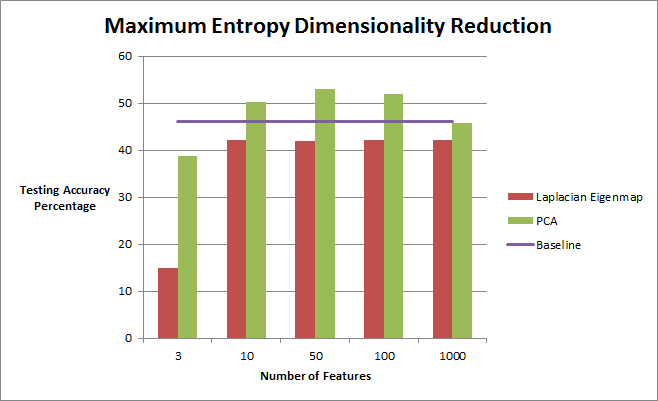
\includegraphics[width=0.7\textwidth]{Maximum_Entropy_Dimensionality_Reduction.png}
\end{center}
\end{figure}

\begin{figure}[!h]
\begin{center}
\caption{SVM with Dimensionality Reduction Testing Accuracy}
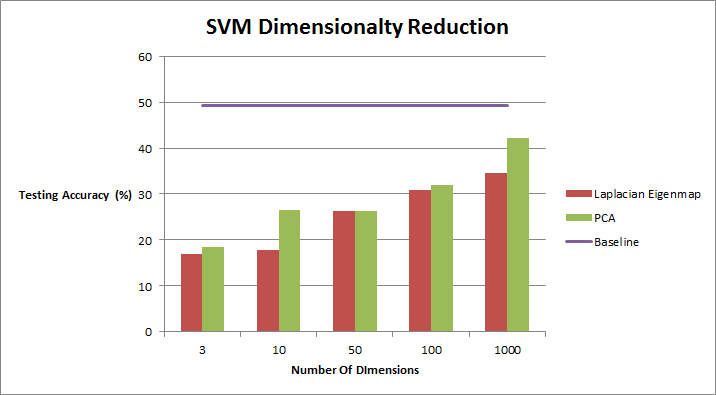
\includegraphics[width=0.7\textwidth]{SVM_Dimensionality_Reduction.png}
\end{center}
\end{figure}

\subsection{Dataset Size}
For the third set of experiments we wanted to determine to what extent more data would begin to alter the accuracy the algorithms.  We use the the jagged-20000 and jagged-40000 datasets which each included description-unigrams.

\begin{table}[Ht]
\caption{Testing Accuracy with \emph{description-unigrams} features}
\centering
\begin{tabular}{| r | c | c |}
\hline
Dataset & SVM & Maximum Entropy \\ \hline
\emph{even-3500} & 49.33\% & 46.12\% \\ \hline
\emph{jagged-20000} & ? & ? \\ \hline
\emph{jagged-40000} & 69.53\% & 69.75\% \\ \hline
\end{tabular}
\end{table}
%\end{figure}

\subsection{Abstract Bigrams}
For the fourth experiment, the jagged-40000 dataset was used with abstract-bigrams used as the features.  The results indicate that the support vector machine had an accuracy of 72.12\% and the maximum entropy algorithm had an accuracy of 72.57\%.  Overall, this is a slight improvement from experiment 3 of 3\% for the support vector machine and an increase of 3\% for the maximum entropy classifier.

\begin{figure}[!h]
\begin{center}
\caption{SVM with Dimensionality Reduction Testing Accuracy}
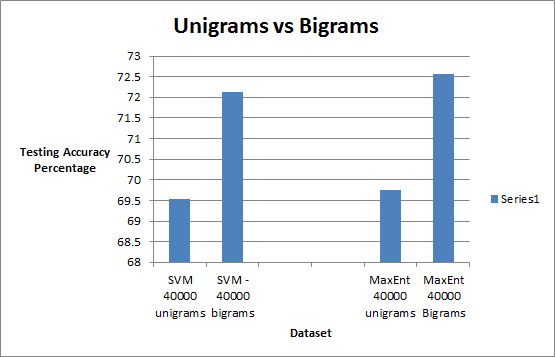
\includegraphics[width=0.7\textwidth]{Unigrams_vs_Bigrams.png}
\end{center}
\end{figure}


\subsection{TfIDF}

